\section{Experimental Results}
\begin{figure*}[t]
\centering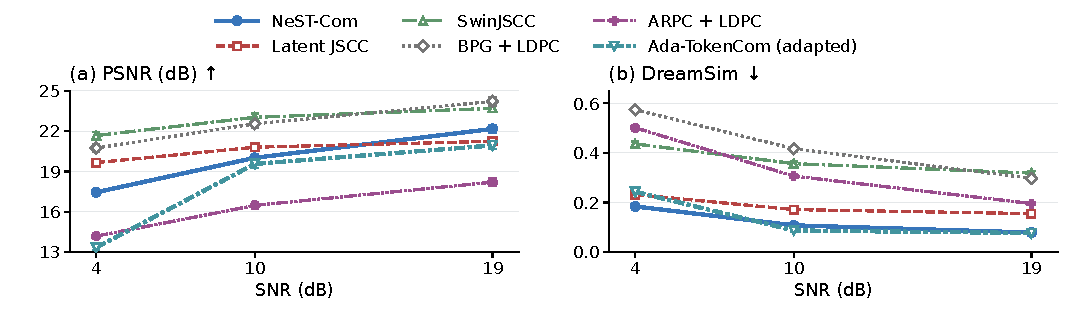
\includegraphics[width=\textwidth]{figure2.pdf}
\caption{Six-system performance on common500 at $N=1024$. Points and bars are source means and pointwise 95\% source-bootstrap CIs after averaging three channel realizations. Ada denotes the predicted-class, fixed-frame adaptation. Higher PSNR and lower DreamSim are favorable.}
\label{fig:performance}
\end{figure*}
\subsection{Experimental Setup}
We use common500 ImageNet validation images~\cite{imagenet}, a disjoint 1000-image calibration set, and the 24 Kodak images~\cite{kodak}, with fixed $256\times256$ preprocessing. Tests use $N=1024$, $E_s=2$, and 4/10/19~dB. ImageNet-calibrated policies remain fixed on Kodak.

The six systems are NeST-Com, Latent JSCC, adapted SwinJSCC~\cite{swinjscc}, adaptive BPG~\cite{bpg} + LDPC, adapted ARPC~\cite{arpc} + LDPC, and Ada-TokenCom adapted to a fixed per-image frame. Our convolutional Latent JSCC maps tokenizer latents to symbols and shares $\Dc$; its losses combine image MSE, LPIPS, and normalized-latent consistency. Latent JSCC and SwinJSCC use the same 20\,000 training images and final 100k/200k-update checkpoints. SwinJSCC was still improving at its training budget cap. All required signaling is charged; ARPC's caption is paid. Ada retains LlamaGen-L/VQ16, prefix arithmetic coding, and conditional tail sampling. A fixed ConvNeXt predicts the class, whose 10-bit ID is transmitted, giving $b+39\leq k_a$. Calibration chooses its MCS; online fitting searches the predeclared 1--256-token endpoints. This changes Ada's average-resource formulation to our fixed-frame task.

Metrics are PSNR, LPIPS-Alex~\cite{lpips}, DreamSim~\cite{dreamsim}, and CLIP-I, the CLIP ViT-L/14 image--image cosine~\cite{clip}. DreamSim/CLIP use frozen FP32, $224\times224$ preprocessing. We average three channel realizations per source, retaining gray failures, then compute equal-source means. Intervals are 95\% source-bootstrap CIs; differences are directly source-paired. Pairing does not require identical noise realizations across methods. Generative seeds and decoding settings are fixed.

\begin{figure*}[t]
\centering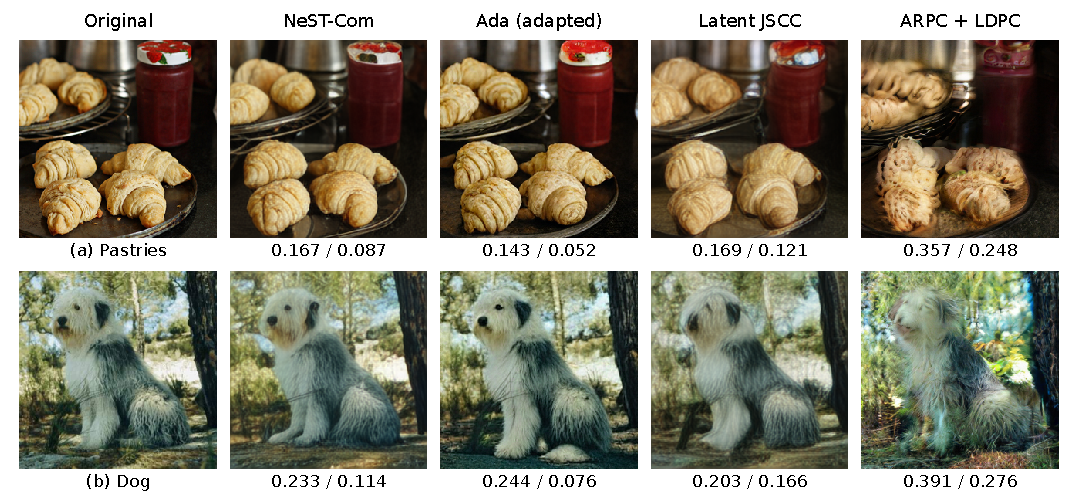
\includegraphics[width=\textwidth]{figure3.pdf}
\caption{Selected methods on two fixed development examples at $N=1024$ and 10~dB: (a) pastries and (b) a dog. Values below each reconstruction are LPIPS-Alex$\downarrow$ / DreamSim$\downarrow$ for that displayed realization.}
\label{fig:qualitative}
\end{figure*}
\subsection{Effect of Within-Scale Endpoints}
\begin{table}[t]
\caption{Within-scale endpoint evidence. (A) Main family-specific policies; $\Delta=\mathrm{PARTIAL}-\mathrm{WHOLE}$ with source-paired 95\% CIs. (B) Controlled 100-source diagnostic at 10 dB.}
\label{tab:internal}
\centering\footnotesize
\setlength{\tabcolsep}{3pt}
\begin{tabular}{ccc}
\toprule
\multicolumn{3}{l}{(A) Main policies: utilization and paired PSNR gain} \\
SNR & Utilization W$\to$P (\%) & $\Delta$PSNR (dB) [95\% CI] \\
\midrule
\multicolumn{3}{l}{common500} \\
4 & 73.81 $\to$ 93.08 & $+0.616\;[0.564,0.673]$ \\
10 & 77.70 $\to$ 95.21 & $+0.701\;[0.637,0.766]$ \\
19 & 85.24 $\to$ 94.73 & $+0.319\;[0.290,0.349]$ \\
\multicolumn{3}{l}{Kodak24} \\
4 & 75.69 $\to$ 93.43 & $+0.396\;[0.236,0.543]$ \\
10 & 78.11 $\to$ 94.99 & $+0.674\;[0.408,0.958]$ \\
19 & 85.69 $\to$ 93.71 & $+0.228\;[0.140,0.324]$ \\
\midrule
\multicolumn{3}{l}{(B) Fixed model, MCS, maximum endpoint and fitting} \\
Grid (candidates) & Utilization (\%) & PSNR (dB) \\
Whole (7) & 78.15 & 18.952 \\
Half (13) & 89.21 & 19.396 \\
Quarter (25) & 95.38 & 19.612 \\
Eighth (49) & 97.39 & 19.735 \\
\bottomrule
\end{tabular}
\end{table}

Table~\ref{tab:internal}(A) compares WHOLE/PARTIAL with shared tokenizer, prior, entropy coder, and $\Dc$. Their target/fallback policies are calibrated separately and select the same MCS at each SNR. On common500, PSNR gains are 0.32--0.70~dB. At 10~dB, utilization rises from 77.70\% to 95.21\% and DreamSim decreases by 0.0240. Kodak gains 0.674~dB and reduces DreamSim by 0.0164 at 10~dB; its 19~dB DreamSim CI includes zero. These results connect additional legal endpoints and calibrated fitting to better use of a fixed body capacity.

Block~B isolates granularity on 100 existing sources, holding model, MCS, maximum endpoint, and longest-feasible fitting fixed. WHOLE, half-, quarter-, and eighth-scale grids have 7/13/25/49 candidates. At 10~dB, QUARTER minus WHOLE gains $0.660\,[0.515,0.814]$~dB, while EIGHTH adds $0.123\,[0.079,0.169]$~dB over QUARTER. The denser grid also yields small PSNR/LPIPS gains at other SNRs; the main quarter grid remains the predefined configuration.

A receiver diagnostic on the same 100 sources separates direct boundary-residual correction from its propagation to finer scales. At 10~dB these contributions are respectively 0.220 and 0.440~dB. Propagation contributes zero at 19~dB, where the boundary is the last scale. These are mechanism diagnostics within the existing population.

\subsection{Comparison With Existing Methods}
\begin{table}[t]
\caption{Perceptual distance and image-feature similarity on common500. Each cell is LPIPS-Alex $\downarrow$ / CLIP-I $\uparrow$.}
\label{tab:external}
\centering\footnotesize
\setlength{\tabcolsep}{3pt}
\begin{tabular}{lccc}
\toprule Method & 4 dB & 10 dB & 19 dB \\
\midrule
NeST-Com & 0.263 / 0.821 & 0.171 / 0.873 & 0.118 / 0.900 \\
Latent JSCC & 0.219 / 0.741 & 0.173 / 0.789 & 0.158 / 0.804 \\
SwinJSCC & 0.530 / 0.627 & 0.469 / 0.669 & 0.440 / 0.697 \\
BPG + LDPC & 0.725 / 0.586 & 0.589 / 0.635 & 0.458 / 0.684 \\
ARPC + LDPC & 0.512 / 0.644 & 0.341 / 0.713 & 0.250 / 0.788 \\
Ada (adapted) & 0.395 / 0.828 & 0.167 / 0.884 & 0.138 / 0.892 \\
\bottomrule
\end{tabular}
\end{table}

Fig.~\ref{fig:performance} and Table~\ref{tab:external} show a quality tradeoff. NeST-Com exceeds adapted Ada in PSNR by 4.116/0.455/1.226~dB at 4/10/19~dB, respectively. At 10~dB, Ada has lower LPIPS and DreamSim and higher CLIP-I, with source-paired CIs excluding zero. Ada also has higher CLIP-I at 4~dB and slightly lower DreamSim at 19~dB; NeST has better PSNR, LPIPS, and CLIP-I at 19~dB. Ada delivers all 256 tokens at 19~dB, so no tail sampling occurs; its approximately 58\% source-capacity utilization reflects completion of its representation.

SwinJSCC and BPG have higher PSNR than NeST at every tested SNR. Latent JSCC has higher PSNR at 4/10~dB and lower LPIPS at 4~dB. Thus perceptual criteria and pixel error need not rank systems alike. NeST's PSNR advantage over ARPC is 3.26--3.97~dB. On matched100, replacing ARPC's original sampling by argmax or a predefined lower temperature changes mean PSNR by up to about 0.15~dB in the tested conditions.

Fig.~\ref{fig:qualitative} shows two selected development examples. Ada retains crisp pastry folds and dog fur; NeST and Latent JSCC smooth different details, while ARPC changes visible object contours and texture. For the dog, Latent JSCC has the lowest displayed LPIPS, whereas Ada has the lowest DreamSim. These individual outcomes complement the source-level comparison.

\subsection{Additional Results and Processing Cost}
On Kodak, all four paired metrics favor NeST over Ada at 4~dB. Only PSNR has a nonzero paired difference at 10~dB; at 19~dB, PSNR and LPIPS favor NeST while DreamSim/CLIP-I CIs cross zero.

The existing $N=2048$ comparison uses 100 sources and two paid 1024-symbol subframes. Its 4/10~dB conditions are adaptive, whereas 19~dB delivers both complete representations. At 19~dB, NeST exceeds ARPC by 1.806~dB PSNR, but ARPC has better DISTS~\cite{dists}: NeST minus ARPC is $+0.0054\,[+0.0024,+0.0086]$. Representation and decoding therefore remain relevant beyond payload fitting.

Measured software processing latency at 10~dB averages 619.71~ms/image for NeST, 42.48 for Latent JSCC, 44.69 for SwinJSCC, 1520.30 for ARPC, and 2293.01 for BPG (RTX PRO~6000, six CPU cores, batch one, 16 development images measured three times after warm-up). These totals sum TX/RX software processing; Ada has not been timed under this protocol.
